% =========================================================================
% SciPost LaTeX template
% Version 2021-08
%
% Submissions to SciPost Journals should make use of this template.
%
% INSTRUCTIONS: simply look for the `TODO:' tokens and adapt your file.
%
% You can also make use of our empty "skeleton" templates for each Journal,
% e.g. SciPostPhys_skeleton.tex
% =========================================================================


% TODO: uncomment ONE of the class declarations below

% Class declaration format: \documentclass[submission, {DOI label of journal}]{SciPost}
% where the DOI label of the journal should be one of:
% Phys          (for SciPost Physics)
% PhysCore      (for SciPost Physics Core)
% PhysLectNotes (for SciPost Physics Lecture Notes)
% PhysProc      (for SciPost Physics Proceedings -> !! Please use the conference-specific template which you will find on our website !!
% PhysCodeb     (for SciPost Physics Codebases)
% Astro         (for SciPost Astronomy)
% Bio           (for SciPost Biology)
% Chem          (for SciPost Chemistry)
% CompSci       (for SciPost Computer Science)
% Math          (for SciPost Mathematics)


%% PHYSICS:
% If you are submitting a paper to SciPost Physics: uncomment next line
%\documentclass[submission, Phys]{SciPost}
% If you are submitting a paper to SciPost Physics Core: uncomment next line
%\documentclass[submission, PhysCore]{SciPost}
% If you are submitting a paper to SciPost Physics Lecture Notes: uncomment next line
\documentclass[submission, PhysLectNotes]{SciPost}
% If you are submitting a paper to SciPost Physics Proceedings: uncomment next line
%\documentclass[submission, PhysProc]{SciPost}
% If you are submitting a paper to SciPost Physics Codebases: uncomment next line
%\documentclass[submission, PhysCodeb]{SciPost}



% Prevent all line breaks in inline equations.
\binoppenalty=10000
\relpenalty=10000

\hypersetup{
    colorlinks,
    linkcolor={red!50!black},
    citecolor={blue!50!black},
    urlcolor={blue!80!black}
}

\usepackage[bitstream-charter]{mathdesign}
\usepackage{amsmath}
\urlstyle{sf}
\usepackage{tikz}
\usepackage{simpler-wick, physics}
\usepackage{epigraph} 

% Fix \cal and \mathcal characters look (so it's not the same as \mathscr)
\DeclareSymbolFont{usualmathcal}{OMS}{cmsy}{m}{n}
\DeclareSymbolFontAlphabet{\mathcal}{usualmathcal}

\DeclareMathOperator{\Ima}{Im}

\begin{document}

% TODO: write your article's title here.
% The article title is centered, Large boldface, and should fit in two lines
\begin{center}{\Large \textbf{
Notes for  the reading club\\
}}\end{center}

% TODO: write the author list here. Use first name (+ other initials) + surname format.
% Separate subsequent authors by a comma, omit comma and use "and" for the last author.
% Mark the corresponding author with a superscript star.
\begin{center}
Reading Club%\textsuperscript{1},
%Aah B. Cee\textsuperscript{2} and
%Gee K. See\textsuperscript{3$\star$}
\end{center}

% TODO: write all affiliations here.
% Format: institute, city, country
\begin{center}
%{\bf 1} Affiliation1
%\\
%{\bf 2} Affiliation2
%\\
%{\bf 3} Affiliation2
%\\
% TODO: provide email address of corresponding author
%${}^\star$ {\small \sf CorrespondingAuthor@email.address}
\end{center}

\begin{center}
\today
\end{center}

% For convenience during refereeing (optional),
% you can turn on line numbers by uncommenting the next line:
%\linenumbers
% You should run LaTeX twice in order for the line numbers to appear.

\section*{Abstract}
{\bf
The Yellow Book Notes. It is good to write notes!
}


% TODO: include a table of contents (optional)
% Guideline: if your paper is longer that 6 pages, include a TOC
% To remove the TOC, simply cut the following block
\vspace{10pt}
\noindent\rule{\textwidth}{1pt}
\tableofcontents\thispagestyle{fancy}
\noindent\rule{\textwidth}{1pt}
\vspace{10pt}


\section{Preliminary}
\subsection{Conventions}
{\it Metric tensor and Coordinate.--}  The metric tensor in Minkowski and Eclidean space-time is defined as
\begin{equation}
    \eta = \begin{Bmatrix}
        +1 &   &\\
           & -1& \\
           &   & ...
    \end{Bmatrix}
\end{equation}
and
\begin{equation}
    \eta = \begin{Bmatrix}
        +1 &   &\\
           & +1& \\
           &   & ...
    \end{Bmatrix}
\end{equation}
respectively, where the first index is the time. In the Yellow Book, without specifications, we are working in Eclidean space. The coordinate is defined as $x^\mu = \{t, \mathop{x}\limits^\rightarrow\}$. So that the norm of a vector in Minkowski space-time is $x^\mu x_\mu = t^2 - r^2$.

{\it $\gamma$ matrices.--}   The $\gamma$ matrices follow the Clifford algebra
\begin{equation}
    \{\gamma^a,\gamma^b\} = 2\eta^{ab}.
\end{equation}
In Minkowski space time, the $\gamma$ matrices can be chosen as
\begin{eqnarray}
    \gamma^0 &=& \sigma^x \nonumber \\
    \gamma^1 &=&  -i\sigma^y,
\end{eqnarray}
while in Elidean space, they can be chosen as
\begin{eqnarray}
    \gamma^0 &=& \sigma^x \nonumber \\
    \gamma^1 &=& \sigma^y.
\end{eqnarray}


\subsection{Free fermions}
In Minkowski space time, the Lagrange density for the free fermion reads
\begin{equation}
    \mathcal{L} = \frac{g}{2}\left(\psi^1\ i(\partial t + \partial x)\ \psi^1 + \psi^2\ i(\partial t - \partial x)\ \psi^2 \right).
\end{equation}
In terms of $\psi = (\psi^1,\psi^2)$, one can write the theory as
\begin{eqnarray}
    \mathcal{L} &=& \frac{g}{2} \left ( \ \psi^\dagger i\partial_t \psi + \psi^\dagger \ \sigma^z \ i\partial_x \psi \ \right) \nonumber \\
    &=& \frac{g}{2} \left ( \ \psi^\dagger \sigma^x\sigma^x i\partial_t \psi + \psi^\dagger \ -i\sigma^x\sigma^y \ i\partial_x \psi \ \right) \nonumber\\
    &=& \frac{g}{2} \psi^\dagger \sigma^x \left(\sigma^x i \partial_t - i\sigma^y i\partial_x \right) \psi \nonumber \\
    &=& \frac{g}{2} \psi^\dagger \gamma^0 i\gamma^\mu \partial_\mu \psi
\end{eqnarray}
where we used 
\begin{equation}
    \gamma^0 = \sigma^x \quad \gamma^1 = -i\sigma^y
\end{equation}

\subsubsection{Wick rotation}
It is usually more convenient to work in Euclidean space rather than Minkowski space time. Upon doing the Wick rotation, the action changes as 
\begin{equation}
    i\ S_M \rightarrow -\ S_E.
\end{equation}
Specifically, 
\begin{eqnarray}
    i\ S[\psi] &=& i\ \int dxdt \ \frac{g}{2} \psi^\dagger \gamma^0 i\gamma^\mu \partial_\mu \psi \nonumber \\
    &=& i^2 \ \int dxdt \ \frac{g}{2} \psi^\dagger \partial_t \psi + i^2 \ \int dxdt \ \frac{g}{2} \psi^\dagger \sigma^x (-i) \sigma^y \partial_x \psi \nonumber \\
    &=& -\int dxd\tau \ \frac{g}{2} \psi^\dagger \partial_\tau \psi - \int dxd(-i t) \ \frac{g}{2} \psi^\dagger \sigma^x \sigma^y \partial_x \psi \nonumber \\
    &=&  -\int dxd\tau \ \frac{g}{2} \psi^\dagger \sigma^x\sigma^x\partial_\tau \psi - \int dxd\tau \ \frac{g}{2} \psi^\dagger \sigma^x \sigma^y \partial_x \psi \nonumber \\
    &=&  -\int dxd\tau \ \frac{g}{2} \psi^\dagger \gamma^0_E\gamma^\mu_E\partial_\mu \psi
\end{eqnarray}
where $\tau = -it$. The Eulidean space action can be written as
\begin{equation}
    S_E = \int d^2x \frac{g}{2} \ \psi^\dagger \gamma^0_E\gamma^\mu_E\partial_\mu \psi
\end{equation}

\subsubsection{1+1d free fermions: Legendre transformation: from $\mathcal{L}$ to H}
A lattice version free fermion theory Eq.~$2.38$ reads
\begin{equation}
    \mathcal{L} = \frac{i}{2} \sum_n \left( \psi_n \dot{\psi_n} + \psi_n \psi_{n+1}\right).
\end{equation}
The canonical momentum corresponding to $\psi_n$ is 
\begin{equation}
    \pi_n = \frac{\partial \mathcal{L}}{\partial \dot{\psi_n}} = -\frac{i}{2}\psi_n.
\end{equation}
So that the Hamiltonian is 
\begin{eqnarray}
    \mathcal{H} &=& \sum_n \pi_n \dot{\psi_n} - \mathcal{L} \nonumber\\
      &=& -\frac{i}{2}\sum_n\psi_n \dot{\psi_n} - \frac{i}{2} \sum_n \left( \psi_n \dot{\psi_n} + \psi_n \psi_{n+1}\right) \\
      &=& -i \sum_n\psi_n \dot{\psi_n} - \frac{i}{2} \sum_n \psi_n \psi_{n+1} \nonumber.
\end{eqnarray}
While it shoud be 
\begin{equation}
    \mathcal{H} = -\frac{i}{2}\sum_n\psi_n \psi_{n+1}.
\end{equation}
If we'd like to keep defining the derivative of Grassmann number according to the order of left-to-right, we need to define the Hamiltonian as
\begin{equation}
    \mathcal{H} = \sum_n \dot{\psi_n} \pi_n - \mathcal{L} =  - \frac{i}{2} \sum_n \psi_n \psi_{n+1}
\end{equation}

\subsection{Free boson}
The action for the free boson in the Minkoswki space time reads
\begin{equation}
    S = \frac{1}{2}g\int \ dxdt \ \partial_\mu \phi \partial^\mu \phi,
\end{equation}
where $\phi$ is a real scalar field. After Wick rotation $\tau = it$, it becomes
\begin{eqnarray}
    i\ S &=& \frac{i}{2}g\int \ dxdt \ \partial_t \phi \partial_t \phi - \frac{i}{2}g\int \ dxdt \ \partial_x \phi \partial_x \phi \nonumber \\
    &=& -\frac{1}{2}g\int \ dxd\tau \ \partial_\tau \phi \partial_\tau \phi - \frac{1}{2}g\int \ dxdit \ \partial_x \phi \partial_x \phi \nonumber \\
    &=& -\frac{1}{2}g\int \ dxd\tau \ \partial_\mu \phi \partial^\mu \phi
\end{eqnarray}
The Euclidean action reads
\begin{equation}
    S_E = \frac{1}{2}g\int \ d^2x \ \partial_\mu \phi \partial^\mu \phi.
\end{equation}
The two point correlation up to a constant term is
\begin{equation}
    \langle \phi(x) \phi(y) \rangle = -\frac{1}{2\pi g} \mathrm{ln} (\rho).
\end{equation}

\subsection{Symmetries at the classical level}
The action becomes different after a coordinate transformation. We say it has a symmetry if it remains unchanged and a Noether current can be derived from the symmetry. The coordinate transformation is denoted as
\begin{equation}
    x'^\mu = x^\mu + \omega_a \frac{\delta x^\mu}{\delta \omega_a}
\end{equation}
and the field changes according to 
\begin{equation}
    \phi'(x') = \phi(x) + \omega_a \frac{\delta F}{\delta \omega_a}(x)
\end{equation}
where $\omega_a$ is a constant and small parameter.

By definition, the change of the action $\delta S$ disappears for a symmetric transformation. We can get nothing new from this. If we allow $\omega_a$ to be arbitrary, the leading contribution to $\delta S$ becomes
\begin{equation}
    \delta S = -\int d^2x j^\mu \partial_\mu \omega_a,  
\end{equation}
where we introduced the the current $j^\mu$. We assume it decreases fast when approaching infinite. So that one obtains 
\begin{equation}
    \delta S = \int d^2x\ \partial_\mu j^\mu \ \omega_a.
\end{equation}
This equations holds for all the field configurations. If we require the field configuration to be the one obeying the equation, the action should be invariant for arbitrary coordinate transformation and one finds the conservation of $j^\mu$
\begin{equation}
    \partial_\mu j^\mu = 0.
\end{equation}

\subsubsection{Energy-momentum tensor}
The canonical energy-momentum tensor is defined to be the Noether current of the translation transformation
\begin{eqnarray}
    x'^\mu &=& x^\mu + \epsilon^\nu \delta^\mu_\nu \\
    T^{\mu\nu} &=& -\eta^{\mu\nu} L + \frac{\partial L}{\partial(\partial_\mu \phi)}\partial_\nu \phi.
\end{eqnarray}
This definition of $T^{\mu\nu}$ is not guaranteed to be symmetric between the two indices (The requirement of a symmetric $T^{\mu\nu}$ will be clear later). 

Another definition that makes the energy-momentum tensor symmetric follows. In the coordinate transformation, if we also consider the variance of the metric tensor 
\begin{equation}
\delta g_{\mu\nu} = -\partial_\mu\epsilon_\nu -\partial_\nu\epsilon_\mu
\end{equation}
the action remains invariant since this is nothing but a reparametrization of the theory. So that one finds
\begin{equation}
    \delta S = 0 = -\frac{1}{2} \int d^dx \ \left(\partial_\mu\epsilon_\nu + \partial_\nu\epsilon_\mu\right) \left(T^{\mu\nu} +2\frac{\delta S}{\delta g_{\mu\nu}}\right).
\end{equation}
So that one can define the energy-momentum tensor as
\begin{equation}
    T^{\mu\nu} = -2\frac{\delta S}{\delta g_{\mu\nu}}
\end{equation}
up to a surface term.

Another way to make the energy-momentum tensor symmetric is add a surface term to the canonical one. One can show that with rotation symmetry, such a term can be constructed to make $T^{\mu\nu}$ symmetric.

\subsection{Symmetry at the quantum level}
All the field configurations contribute to the quantum theory, so that one has no Noether current in general. Still the symmetry has constraints to the quantum theory. For the $n-$point correlation functions, one has
\begin{eqnarray}
\langle \phi(x'_1)...\phi(x'_n) \rangle &=& \frac{1}{Z}\int [D\phi]\ \phi(x'_1)...\phi(x'_n) \ e^{-S[\phi]} \\
&=& \frac{1}{Z}\int [D\phi']\ \phi'(x'_1)...\phi'(x'_n) \ e^{-S'[\phi']} \\
&=& \frac{1}{Z}\int [D\phi]\ F(\phi(x_1))...F(\phi(x_n)) \ e^{-S[\phi]} \\
&=& \langle\ F(\phi(x_1))...F(\phi(x_n)) \ \rangle
\end{eqnarray}
in which we assumed the functional integral measure does not change and the coordinate transformation is a rigid one ($\omega_a$ is a constant).
\subsubsection{Ward identity}
As stated above there is no conserved current at the quantum level. The infinitesimal coordinate transformation at the quantum level results in the so-called Ward identity.

We denote the change of fields as
\begin{equation}
    \phi'(x) = \phi(x) -i\omega_a\ G_a\ \phi(x).
\end{equation}
The infinitesimal coordinate transformation ($\omega_a$ now is arbitrary) changes the correlation as (We only consider the first order perturbation contribution) 
\begin{eqnarray}
\langle \phi'(x_1)... \phi'(x_n)\rangle &=& \langle \phi(x_1)... \phi(x_n)\rangle \\ 
&=& \frac{1}{Z} \int [D\phi'] (X+\delta X) e^{-S[\phi] - \int d^dx\partial_\mu j^\mu \omega_a} \\
&=& \frac{1}{Z} \int [D\phi] (X+\delta X) e^{-S[\phi] - \int d^dx\partial_\mu j^\mu \omega_a} \\
&=& \langle X \rangle - \int [D\phi] \int d^dx\ X \partial_\mu j^\mu \omega_a e^{-S[\phi]} - \int [D\phi] \delta X  e^{-S[\phi]}
\end{eqnarray}
so that one finds
\begin{equation}
    \langle\delta X\rangle = \int d^dx \ \partial_\mu\langle j^\mu \ X\rangle \omega_a(x).
\end{equation}
As
\begin{eqnarray}
\delta X &=& -i \sum_i \phi(x_1)...G_a \phi(x_i)...\phi(x_n)\omega_a(x_i) \\
&=& -i \int d^dx \sum_i \phi(x_1)...G_a \phi(x_i)...\phi(x_n)\delta(x-x_i)\omega_a(x)
\end{eqnarray}
Since $\omega_a$ is arbitrary, one obtains the Ward identity
\begin{equation}
    \partial_\mu\langle j^\mu \ X\rangle = -i \sum_i \delta(x-x_i)\ \langle \phi(x_1)...G_a \phi(x_i)...\phi(x_n).
\end{equation}
So that for each symmetry, there exists a Ward identity, i.e., a constraint to the correlation function. With enough symmetries, one can get all the information of the correlation functions.

\subsection{Renormalization group}
\subsubsection{Dimensional analysis and renormalizability of QFT}
Let's start with the canonical dimension of fields and couplings in the action,
\begin{equation}
    S = \int d^dx \ \mathcal{L}(\phi, \lambda).
\end{equation}
Since the action is dimensionless, every term in $\mathcal{L}$ has an energy scaling dimension of
\begin{equation}
    \Delta(\mathcal{L}) = [\mathcal{L}] = \omega^d
\end{equation}
which determines the canonical dimension fields and couplings. The renormalizability of a QFT is directly obtained from the energy dimension of Feynman diagrams,
\begin{equation}
    \mathcal{D} = d - E_{\phi} \Delta (\phi) - \Delta (\lambda_i)
\end{equation}
where $E_{\phi}$ is the number of external fields and $\lambda_i$ the couplings in the theory. A nice discussion about renormalizability can be found online (https://web2.ph.utexas.edu/~vadim/
Classes/2022f/notes.html).

Super-renormalizable theories have only couplings with positive dimensions. For such theories, there are finite Feynman diagrams become divergent in the perturbation calculation. Renormalizable theories have couplings with non-negative dimensions, in which a finite number of couplings have zero dimensions. There exists infinite number of divergent Feynman diagrams, but the number of divergent amplitudes is finite. If there is at least one coupling with a negative dimension, the theory is non-renormalizable.

\subsubsection{Wilson-Kadanoff renormalization scheme}
The renormalization group builds up the modern understanding of QFT, which is regarded as an effective field theory. Here we briefly recall the Wilson-Kadanoff scheme. In this scheme, a momentum cutoff $\boldsymbol{k}<\Lambda$ is introduced. 

One first divides modes into fast $\Lambda/s<\boldsymbol{k}<\Lambda$ and slow $\boldsymbol{k}<\Lambda/s$ parts. The fast modes are integrated to result in a new theory 
\begin{equation}
    e^{-S'(\phi)_{\Lambda/s}} = \int \mathrm{D}\phi_{\Lambda/s<\boldsymbol{k}<\Lambda} \ e^{-S_{\Lambda}(\phi)}
\end{equation}
with a smaller cutoff $\Lambda/s$. This theory can not be compared with the original theory, since they have different cutoffs. Another rescaling step 
\begin{equation}
    \boldsymbol{k'} = \boldsymbol{k} s
\end{equation}
is required to restore the 

\section{Conformal group in d=2}

In $d=2$ we have infinitely many \emph{local} conformal transformations. The 6 parameter subgroup of conformal transformations that are everywhere well defined is the \emph{global} conformal group $SL(2,\mathbb{C})/\mathbb{Z}_2$.

\section{Normal ordering}
For free fields the OPE of the field with itself contains only one term with a constant prefactor. It can be regularized by normal ordering the fields, or equivalently, subtracting its expectation value.
Using the former prescription for $T(z)T(w)$ only kills the $\propto c$ term. So clearly we need a more elaborate definition of normal ordering. We shall define proper normal ordering for general fields as subtracting all the singular terms from the OPE. We will write this normal ordering as
\begin{equation}
	(AB)(z).
\end{equation}
Concretely, given the OPE
\begin{equation}
	A(z)B(w) = \sum_{n=-\infty}^{N}\frac{\left\{AB\right\}_n(w)}{(z-w)^n}
\end{equation}
we have that
\begin{equation}
	(AB)(w) = \left\{AB\right\}_0(w).
\end{equation}
Equivalently, we can compute the normal ordering of fields using contour integral methods:
\begin{equation}
	(AB)(w) = \frac{1}{2\pi i}\oint \frac{dz}{z-w}A(z)B(w).
\end{equation}
The contraction of fields contains only the singular terms of the OPE:
\begin{equation}
	\wick{\c A(z) \c B(w)} = \sum_{n=1}^N\frac{\left\{AB\right\}_n(w)}{(z-w)^n}.
\end{equation}
We now want to express the modes of the normal ordered field in terms of the modes of the input fields. Given fields $A$ and $B$ and points $|z|>|x|>|w|$ we write
\begin{subequations}
\begin{align}
	A(z) &= \sum_n (z-x)^{-n-h_A}A_n(x) \\
	B(w) &= \sum_n (w-x)^{-n-h_B}B_n(x).
\end{align}
\end{subequations}
Contour integrating ultimately results in:
\begin{equation}
	(AB)_m = \sum_{n\leq -h_A} A_nB_{m-n} + \sum_{n>-h_A}B_{m-n}A_n,
\end{equation}
where we defined the modes of $(AB)$ as:
\begin{equation}
	(AB)(z) = \sum_n z^{-n-h_A-h_B}(AB)_n.
\end{equation}
Some warnings are in place:
\begin{enumerate}
	\item Normal ordering is not commutative: $(AB)(z) \neq (BA)(z)$.
	\item Normal ordering is not associative: $((AB)C)(z)\neq(A(BC))(z)$.
	\item With this definition of normal ordering, Wick's theorem needs to be revisited. This is done in Appendix 6.B of the Book.
\end{enumerate}

\section{Conformal families and Operator algebra}
\epigraph{There's nothing stronger than family.}{D. T.}
The goal of this section is to introduce the notion of conformal blocks and associated to this the method of conformal bootstrapping as a way to solve CFTs, ie. compute the correlation functions, explicitly. Before that we revisit the notion of descendant fields and conformal families.

In the following we mostly only care about the holomorphic part of fields.
\subsection{Descendant fields}
A descendant is generated from a primary by acting with the Virasoro operators:
\begin{equation}
	\phi^{(-n)}(w) = (L_{-n}\phi)(w) = \frac{1}{2\pi i}\oint_w dz \frac{1}{(z-w)^{n-1}}T(z)\phi(w),
\end{equation}
in particular:
\begin{equation}
	\phi^{(0)}(w) = h\phi(w), \qquad \phi^{(-1)} = \partial \phi(w).
\end{equation}
Consider following correlation function of states that are part of the same family:
\begin{equation}
	\expval{(L_{-n}\phi)(w)X},
\end{equation}
where $X$ denotes a string of primary fields: $X=\phi_1(w_1)...\phi_N(w_N)$. After a computation one finds:
\begin{equation}
	\expval{(L_{-n}\phi)(w)X} = \mathcal{L}_{-n}\expval{\phi(w)X} \qquad (n\geq 1).
\end{equation}
With the differential operator
\begin{equation}
	\mathcal{L}_{-n} = \sum_i \left\{ \frac{(n-1)h_i}{(w_i - w)^n} - \frac{1}{(w_i - w)^{n-1}}\partial_{w_i}\right\}.
\end{equation}
In other words, knowing all the correlation functions between primaries, $\expval{\phi(w)X}$, is sufficient to compute the correlation functions that involve descendants by applying the differential operators $\mathcal{L}_{-n}$. More generally, for descendants of the form
\begin{equation}
	\phi^{(-k,-n)}(w) = (L_{-k}L_{-n}\phi)(w),
\end{equation}
and so on, we find in a similar way that
\begin{equation}
	\expval{(L_{-k_1}...L_{-k_n}\phi)(w)X} = \mathcal{L}_{-k_1}...\mathcal{L}_{-k_n}\expval{\phi(w)X} \qquad (n\geq 1)
\end{equation}
\subsection{Conformal families}
A \emph{conformal family} is a set of states that transform according to a representation of the conformal group. A family contains a primary and its descendants. We will denote the conformal family associated with the primary $\phi$ by $[\phi]$. First descendants of a primary are sometimes called \emph{secondary fields}. Another way to say that a conformal family transforms under itself is to say that the OPE of $T(z)$ with any member of the family will be composed solely of other members within the same family. Concretely:
\begin{equation}
	T(z)\phi^{(-n)}(w) = \frac{cn(n^2-1)/12}{(z-w)^{n+2}}\phi(w) + \sum_{k=1}^{n}\frac{n+k}{(z-w)^{k+2}}\phi^{(k-n)}(w) + \sum_{k\geq 0}(z-w)^{k-2}\phi^{(-k,-n)}(w)
\end{equation}
\subsection{The operator algebra}
The two - and three point functions of a CFT are fixed by conformal invariance. However, we need additional dynamical information to compute the three-point fusion coefficients $C_{ijk}$ (for example using a conformal bootstrap approach). This information is contained in the \emph{operator algebra}. The OPE which also includes the regular terms of all primary fields with each other. Using the operator algebra we can reduce all correlation functions to two-point correlation functions.

First we choose a basis of fields such that $C_{\alpha\beta} = \delta_{\alpha\beta}$ in
\begin{equation}
	\expval{\phi_\alpha(w,\overline{w})\phi_\beta(z,\overline{z})} = \frac{C_{\alpha\beta}}{(w-z)^{2h}(\overline{w}-\overline{z})^{2\overline{h}}}.
\end{equation}
This implies that states belonging to different conformal families are always orthogonal.
From scale invariance it follows that:
\begin{equation}
	\phi_1(z,\overline{z})\phi_2(0,0) = \sum_p \sum_{\{k,\overline{k}\}} C_{12}^{p\{k,\overline{k}\}}z^{h_p-h_1 -h_2+K} \overline{z}^{\overline{h}_p-\overline{h}_1-\overline{h}_2+\overline{K}}\phi_p^{(k,\overline{k})}(0,0).
\end{equation}
We introduced the notation $K = \sum_i k_i$.

Writing
\begin{equation}
	C_{12}^{p\{0,0\}} \equiv C^p_{12} = C_{p12},
\end{equation}
we find that
\begin{equation}
	C_{12}^{p\{k,\overline{k}\}} = C_{12}^p \beta_{12}^{p\{k\}} \overline{\beta}_{12}^{p\{\overline{k}\}}.
\end{equation}
This means that descendants fields are correlated to a given third field only if the primary is correlated. An the holomorphic and antiholomorphic parts factorize.

An example is given in the Book. Even in a relatively simple case, finding the three point function is not straightforward!

In conclusion, given the central charge, the conformal dimensions and the three-point coefficients $C_{pnm}$, one can - in principle - determine the operator algebra. Using the operator algebra, all the n-point correlation functions can be computed and the entire theory is solved.

\subsection{Conformal blocks}

Let us illustrate how the four-point functions can be reduced to three-point functions using the machinery introduced in the previous sections.

We consider the four-point function
\begin{equation}
	\expval{\phi_1(z_1,\overline{z}_1)\phi_2(z_2,\overline{z}_2)\phi_3(z_3,\overline{z}_3)\phi_4(z_4,\overline{z}_4)}.
\end{equation}
For sake of simplicity, we shall carry out a global conformal transformation to put $z_4 = 0$, $z_1 = \infty$, $z_2 = 1$, $z_3 = x$.
We define:
\begin{equation}
	G_{34}^{21}(x,\overline{x}) = \mel{h_1,\overline{h}_1}{\phi_2(1,1)\phi_3(x,\overline{x})}{h_4,\overline{h}_4}.
\end{equation}
Note the order of the indices!

Using operator algebra techniques, we can write this function as:
\begin{equation}
	G_{34}^{21}(x,\overline{x}) = \sum_p C_{34}^p C_{12}^p A_{34}^{21}(p|x,\overline{x}).
\end{equation}
The sum over $p$ is a sum over intermediate conformal families that play the role of mediating channels in the scattering from fields from $(0,x)$ towards $(1,\infty)$. These functions $A_{34}^{21}(p|x,\overline{x})$ are called \emph{partial waves}. They can be depicted by:
\begin{figure}[htb]
\centering
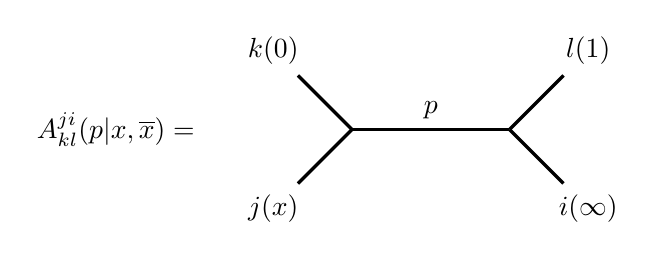
\begin{tikzpicture}[very thick]
	\node at (-1,1) (k) {$k (0)$};
	\node at (-1,-1) (j) {$j (x)$};
	\node at (3,1) (l) {$l (1)$};
	\node at (3,-1) (i) {$i (\infty)$};
	
	\node at (-3,0) {$A_{kl}^{ji}(p|x,\overline{x})=$};
	
	\draw (k) -- (0,0) ;
	\draw (j) -- (0,0);
	\draw (0,0) -- node[above] {$p$} ++ (2,0);
	\draw (2,0) -- (l);
	\draw (2,0) -- (i);
\end{tikzpicture}
\end{figure}

The partial wave factorizes in a holomorphic and antiholomorphic part, according to:
\begin{equation}
	A_{34}^{21}(p|x,\overline{x}) = \mathcal{F}_{34}^{21}(p|x)\overline{\mathcal{F}}_{34}^{21}(p|\overline{x}),
\end{equation}
we call these functions $\mathcal{F}$, the \emph{conformal blocks}. There is a recipe to compute these conformal blocks, even though it is a pain to compute these in practice. Physically speaking, these conformal blocks are the part in the four-point function that is fixed by conformal invariance. They depend on the anharmonic ratios via a series expansion. The remaining elements are the three-point coefficients, which are \emph{not} fixed by conformal invariance.

\subsection{Crossing symmetry and the conformal bootstrap}

What happens if we would choose instead of $z_4 = 0$, $z_1 = \infty$, $z_2 = 1$, $z_3 = x$ a different order of the fields? Following identities can be obtained relatively easy:
\begin{equation}
	G_{34}^{21}(x,\overline{x}) = G_{32}^{41}(1-x,1-\overline{x}),
\end{equation}
and
\begin{equation}
	G_{34}^{21}(x,\overline{x}) = \frac{1}{x^{2h_3}\overline{x}^{2\overline{h}_3}}G_{31}^{24}(1/x,1/\overline{x}).
\end{equation}
These identities are specific instances of the \emph{crossing symmetry} of the functions $G$. Explicitly we can write the first identity as
\begin{equation}
	\sum_p C_{21}^pC_{34}^p\mathcal{F}_{34}^{21}(p|x)\overline{\mathcal{F}}_{34}^{21}(p|\overline{x}) = \sum_q C_{41}^q C_{32}^q \mathcal{F}_{32}^{41}(p|1-x)\overline{\mathcal{F}}_{32}^{41}(p|1-\overline{x}),
\end{equation}
which has a aesthetically pleasing pictorial interpretation:
\begin{figure}
\centering
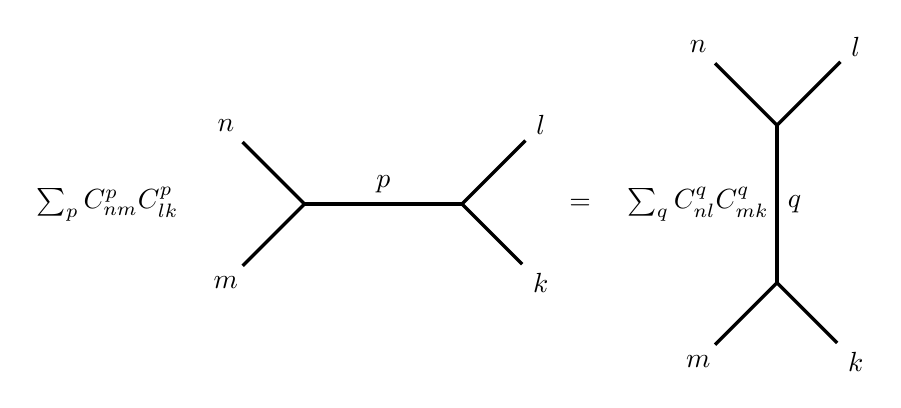
\begin{tikzpicture}[very thick]
\node at (-1,1) (k) {$n$};
\node at (-1,-1) (j) {$m$};
\node at (3,1) (l) {$l$};
\node at (3,-1) (i) {$k$};

\node at (-2.5,0) {$\sum_p C_{nm}^pC_{lk}^p$};

\draw (k) -- (0,0) ;
\draw (j) -- (0,0);
\draw (0,0) -- node[above] {$p$} ++ (2,0);
\draw (2,0) -- (l);
\draw (2,0) -- (i);

\node at (3.5,0) {$=$};

\begin{scope}[shift={(6,-1)}]
\node at (-1,-1) (m) {$m$};
\node at (1,-1) (k) {$k$};
\node at (-1,3) (n) {$n$};
\node at (1,3) (l) {$l$};

\node at (-1,1) {$\sum_q C_{nl}^qC_{mk}^q$};

\draw (m) -- (0,0) ;
\draw (k) -- (0,0);
\draw (0,0) -- node[right] {$q$} ++ (0,2);
\draw (0,2) -- (n);
\draw (0,2) -- (l);
\end{scope}
\end{tikzpicture}
\end{figure}
Crossing symmetry imposes $N^4$ constrains on the $N^3 + N$ parameters $C_{mn}^p$ and $h_p$. Exploiting crossing symmetry to compute these parameters is called \emph{conformal} bootstrap.
\appendix

\section{Central extensions of Lie algebras}
In this section $\mathfrak{g},\mathfrak{h},...$ denote (possibly infinite) Lie algebras over some field $\mathbb{K} = \mathbb{R}, \mathbb{C}$. This section is mainly based on Wikipedia and~\cite{Schottenloher}.
\subsection{Extensions}
{\bf Definition:} A \emph{Lie algebra extension} is a short exact sequence of Lie algebras:
\begin{equation}
	\mathfrak{h}\overset{\iota}{\rightarrow}\mathfrak{e}\overset{\pi}{\rightarrow}\mathfrak{g}.
\end{equation}
One calls $\mathfrak{e}$ an extension of $\mathfrak{g}$ by $\mathfrak{h}$. By exactness of the sequence one has $\mathfrak{g}\cong\mathfrak{e}\slash\Ima\iota$.\\

{\bf Definition:} A \emph{central extension} is an extension $\mathfrak{e}$ of $\mathfrak{g}$ by $\mathfrak{h}$, such that $\Ima \iota$ is contained in the center of $\mathfrak{e}$, $\iota(\mathfrak{h})\subseteq Z(\mathfrak{e})$.\\

Notice that for a central extension $\mathfrak{h}$ is necessarily abelian. We now introduce a notion of trivial central extensions as follows:

{\bf Definition:} A Lie algebra extension
\begin{equation}
	\mathfrak{h}\overset{\iota}{\rightarrow}\mathfrak{e}\overset{\pi}{\rightarrow}\mathfrak{g}
\end{equation}
\emph{splits} if there exists a Lie algebra morphism $\beta: \mathfrak{g}\mapsto\mathfrak{e}$ such that $\pi\circ\beta = \text{id}_{\mathfrak{e}}$. $\beta$ is called a splitting map.\\

A central extension
\begin{equation}
	\mathfrak{h}\overset{\iota}{\rightarrow}\mathfrak{e}\overset{\pi}{\rightarrow}\mathfrak{g}.
\end{equation}
that splits is trivial in the sense that it is equivalent\footnote{To do: introduce the notion of equivalent extensions.} to one where $\mathfrak{e}\cong\mathfrak{g}\oplus\mathfrak{h}$.\\

Let us now consider a central extension and a map (not necesserily a Lie algebra homomorphism) $\beta:\mathfrak{g}\rightarrow\mathfrak{e}$ such that $\pi\circ\beta = \text{id}_{\mathfrak{e}}$. From this map construct
$\Theta: \mathfrak{g}\times\mathfrak{g}\rightarrow\mathfrak{h}$ as follows:
\begin{equation}
	\Theta(x,y) := \left[\Theta(x),\Theta(y)\right] - \Theta\left([x,y]\right).
\end{equation}
This map is:
\begin{enumerate}
	\item \label{prop:antisym} Antisymmetric.
	\item \label{prop:bilinear} Bilinear.
	\item \label{prop:Jacobi} Satisfies $\Theta(x,[y,z]) + \Theta(y,[z,x]) + \Theta(z,[x,y]) = 0$. 
\end{enumerate}
Given $\Theta$ one can now show that there is an isomorphism between the vector spaces $\mathfrak{e}\cong\mathfrak{g}\oplus\mathfrak{h}$ that is given by:
\begin{equation}
	\Psi:\mathfrak{g}\oplus\mathfrak{h}\mapsto\mathfrak{e}:(x,y)\mapsto\beta(x) + y.
\end{equation}
A Lie bracket on $\mathfrak{g}\oplus\mathfrak{h}$ is given by:
\begin{equation}
	[x\oplus z, y\oplus z']_{\mathfrak{e}} := [x,y]_\mathfrak{g} + \Theta(x,y).
\end{equation}

{\bf Lemma:} In the above construction $\beta$ is a splitting map if and only if
\begin{equation}
	\Theta(x,y) = \mu([x,y]),
\end{equation}
for some $\mu\in\text{Hom}(\mathfrak{g},\mathfrak{h})$.\\

Now comes the classification of central extensions of Lie algebras:\\

{\bf Theorem:} Every central extension comes from a map $\Theta$ that satisfies the above properties (\ref{prop:antisym}-\ref{prop:Jacobi}). Conversely, every central extension gives rise to a map $\Theta$ that satisfies the above properties (\ref{prop:antisym}-\ref{prop:Jacobi}).

\subsection{Lie algebra cohomology}
The classification of Lie algebra extensions is very satisfying. It smells a lot like a cohomological classification. Indeed, the extensions are classified by functions depending on two variables satisfying the condition (\ref{prop:Jacobi}) that is exactly the one needed to fulfill the Jacobi identity of the central extension. Moreover, the central extension is trivial if the \emph{2-cocycle} $\Theta$ is trivial in the following sense: $\Theta(x,y) = \mu([x,y])$. This is reminiscent of considering 2-cocycles to be trivial if they are equal to a coboundary. Let us put this on a bit more rigorous footing.\\

{\bf Definitions:}
\begin{enumerate}
	\item $Z^2(\mathfrak{g},\mathfrak{h}) = \left\{\Theta\in\Lambda^2(\mathfrak{g},\mathfrak{h})|\Theta:(\ref{prop:Jacobi})\right\}$.
	\item $B^2(\mathfrak{g},\mathfrak{h})=\left\{\Theta:\mathfrak{g}\times\mathfrak{g}\mapsto\mathfrak{h}|\exists\mu\in\text{Hom}(\mathfrak{g},\mathfrak{h}):\Theta(-,-)=\mu([-,-])\right\}$.
	\item $H^2(\mathfrak{g},\mathfrak{h}):=Z^2(\mathfrak{g},\mathfrak{h})/B^2(\mathfrak{g},\mathfrak{h})$.
\end{enumerate}
$H^2$ is of course called the second cohomology group. We thus obtain the following reformulation of the classification of central extensions:\\

{\bf Theorem:} The equivalence classes of central extensions
\begin{equation}
	\mathfrak{h}\overset{\iota}{\rightarrow}\mathfrak{e}\overset{\pi}{\rightarrow}\mathfrak{g}
\end{equation}
are in one-to-one correspondence with the elements of $H^2(\mathfrak{g},\mathfrak{h})$.\\

For completeness, let us introduce a notion of cochain complexes for Lie algebras. A cochain $f$ is a alternating multilinear map $f$:
\begin{equation}
	f:\Lambda^n \mathfrak{g} \mapsto \mathfrak{h}.
\end{equation}
Here, $\mathfrak{h}$ is considered a $\mathfrak{g}$-module or -representation.

The differential of an $n$-cochain is given by
\begin{equation}
\begin{aligned}
	(d f)\left(x_1, \ldots, x_{n+1}\right) =
	&\sum_i     (-1)^{i+1}x_i\, f\left(x_1, \ldots, \hat x_i, \ldots, x_{n+1}\right) + \\
	&\sum_{i<j} (-1)^{i+j}      f\left(\left[x_i, x_j\right], x_1, \ldots, \hat x_i, \ldots, \hat x_j, \ldots, x_{n+1}\right)\, ,
\end{aligned}
\end{equation}

so for example, with trivial action we obtain
\begin{equation}
	(df)(x_1,x_2) = f([x_1,x_2]),
\end{equation}
and
\begin{equation}
\begin{aligned}
	(df)(x_1,x_2,x_3) &= -f([x_1,x_2],x_3) + f([x_1,x_3],x_2) - f([x_2,x_3],x_1)\\
	&= -f([x_1,x_2],x_3) - f([x_3,x_1],x_2) - f([x_2,x_3],x_1)\\
	&= f(x_3,[x_1,x_2]) + f(x_2,[x_3,x_1]) + f(x_1,[x_2,x_3]).
\end{aligned}
\end{equation}
So clearly, $Z^2(\mathfrak{g},\mathfrak{h})$ defined above is the group of 2-cocycles satisfying $d\Theta=0$ and $B^2(\mathfrak{g},\mathfrak{h})$ the set of coboundaries: $\Theta = d\mu$.
\bibliography{refs.bib}

\nolinenumbers

\end{document}
